\chapter{Allegati}
Tutto il codice è disponibile su github.

Il software all'indirizzo: https://github.com/Psykopear/DroneGame

Il sorgente della tesi stessa all'indirizzo: https://github.com/Psykopear/Thesis

\section{Sorgente algoritmo geometrico}
\begin{verbatim}
from utils.direction_modifier import void_directions, get_direction, d
import random


def search_far_calibration(drone):

  distances = drone.distances
  STEP = len(distances)

  # Calibrazione non effettuata

  if STEP <= 2:

    direction = d["E"] if STEP == 1 else d["N"] \
    if STEP == 2 else drone.last_direction
    return void_directions(direction, drone)

  # Calibrazione effettuata, inizio a muovermi

  elif STEP == 3:

    # Le tre misurazioni della "triangolazione" per capire
    # il quadrante in cui si trova il punto d'arrivo

    sud_ovest, sud_est, nord_est = distances[:3]
    direction = "S" if sud_est < nord_est else \
    "N" if sud_est > nord_est else ""
    direction += "E" if sud_ovest > sud_est \
    else "O" if sud_ovest < sud_est else ""
    drone.last_direction = d[direction]

  #Parametro che influenza l'efficenza
  if drone.graph[drone.actual_position[0]][drone.actual_position[1]] >= 3:
    return change_strategy(drone)
  else:
    return go_far(drone)

def go_far(drone):

  if len(drone.distances) > 3 and \
  (drone.distances[-2] - drone.distances[-1]) < 0:

    if drone.last_modifier == 0:

      drone.last_modifier = 1 if random.random() < 0.5 else -1

    if not drone.flipflop:

      drone.flipflop, drone.last_direction = (True, \
      (drone.last_direction + drone.last_modifier) % 8)

    else:

      mod = 3 if drone.distances[-1] > drone.distances[-2] else 1
      drone.flipflop, drone.last_direction = (False, \
      (drone.last_direction + mod) % 8)

  if len(drone.distances) > 3 and (drone.distances[-2] \
  - drone.distances[-1]) > 1 and drone.flipflop:

    drone.flipflop, drone.last_direction = (True, \
    (drone.last_direction - drone.last_modifier) % 8)

  else:

    drone.flipflop = True

  return void_directions(drone.last_direction, drone)


def change_strategy(drone):

  drone.distances = []
  x, y = drone.actual_position
  close_distances = []

  # Controllo in quale dei punti 
  # adiacenti sono passato meno volte

  for x_index in (x - 1, x, x + 1):
    for y_index in (y - 1, y, y + 1):

      # Se il punto e' accessibile, e non e' il punto stesso in 
      # cui sono partito viene aggiunto all'array

      if x_index >= 0 and x_index < len(drone.graph[0]) \
      and y_index >= 0 and y_index < len(drone.graph[0]):
        if x_index != x or y_index != y:

          # Questo array conterra' tutti i punti 
          # adiacenti ed accessibili

          try:
            close_distances.append(\
            [drone.kb[(x_index, y_index)][1], x_index, y_index])
          except:
            close_distances.append([0, x_index, y_index])

  # Vado verso il primo dei punti in cui sono passato meno volte
  return void_directions(get_direction(min(close_distances)[1]\
  - x, min(close_distances)[2] - y), drone)

\end{verbatim}


\section{Sorgente dell'algoritmo ottimo}
\begin{verbatim}
def greedy_generic(drone):

  x, y = drone.actual_position

  available = []

  for x_index in (x - 1, x, x + 1):

    for y_index in (y - 1, y, y + 1):

      if x_index >= 0 and x_index < len(drone.graph[0]) \
      and y_index >= 0 and y_index < len(drone.graph[0]):
        if x_index != x or y_index != y:
          available.append([drone.kb[(x_index, y_index)][0], \
          x_index, y_index])

  go_x, go_y = min(available)[1], min(available)[2]
  return void_directions(get_direction(go_x - x, go_y - y), drone)

\end{verbatim}
	
\section{Sorgente generazione grafo dinamico}
\begin{verbatim}
class Graph(object):

  def __init__(self, x, y):

    self.graph = {}
    self.graph[(x, y)] = (0, 1, 0)
    self.counter = 1

    # Set this to the same amount of Drone.fuel to make
    # the algorithm behave like if there is no optimization
    # If it's less, it will delete nodes when the graph becomes
    # big, saving memory, with a variable increase of the cost
    # of the search algorithm. 20 seemed to be a good choice for
    # this parameter, for matrixes between 5 and 20 of size
    # (obviously not deleting nodes is always better for calculations)

    self.graph_max_length = 2000

  def __getitem__(self, item):

    return self.graph[item]

  def add_node_coord(self, coord):

    self.counter += 1

    if len(self.graph) > self.graph_max_length:

      for node in self.graph:

        if self.graph[node][2] == (self.counter - self.graph_max_length):

          self.graph.pop(node, None)
          break

    new_node = Node(coord, 1, self.counter)

    if not new_node.k in self.graph:

      self.graph[new_node.k] = new_node.v

    else:

      old_node = self.graph[coord]
      self.graph[coord] = (old_node[0], old_node[1] + 1, self.counter)

    return new_node.k

  def change_weight(self, coord, w):

    self.graph[coord] = (w, self.graph[coord][1], self.graph[coord][2])

  def print_graph(self):

    for node in self.graph:

      print node, ": ", self.graph[node]

  def goto(self, coord, way):

    new_coord = sum_coord(coord, d[way])
    return self.graph[new_coord] if new_coord in self.graph else -1


class Node(object):

  def __init__(self, k, weight, counter):

    self.k = k
    self.v = (weight, 1, counter)

\end{verbatim}
\pagebreak
\section{Screenshot iterazioni}

\begin{figure}[hb]
\center
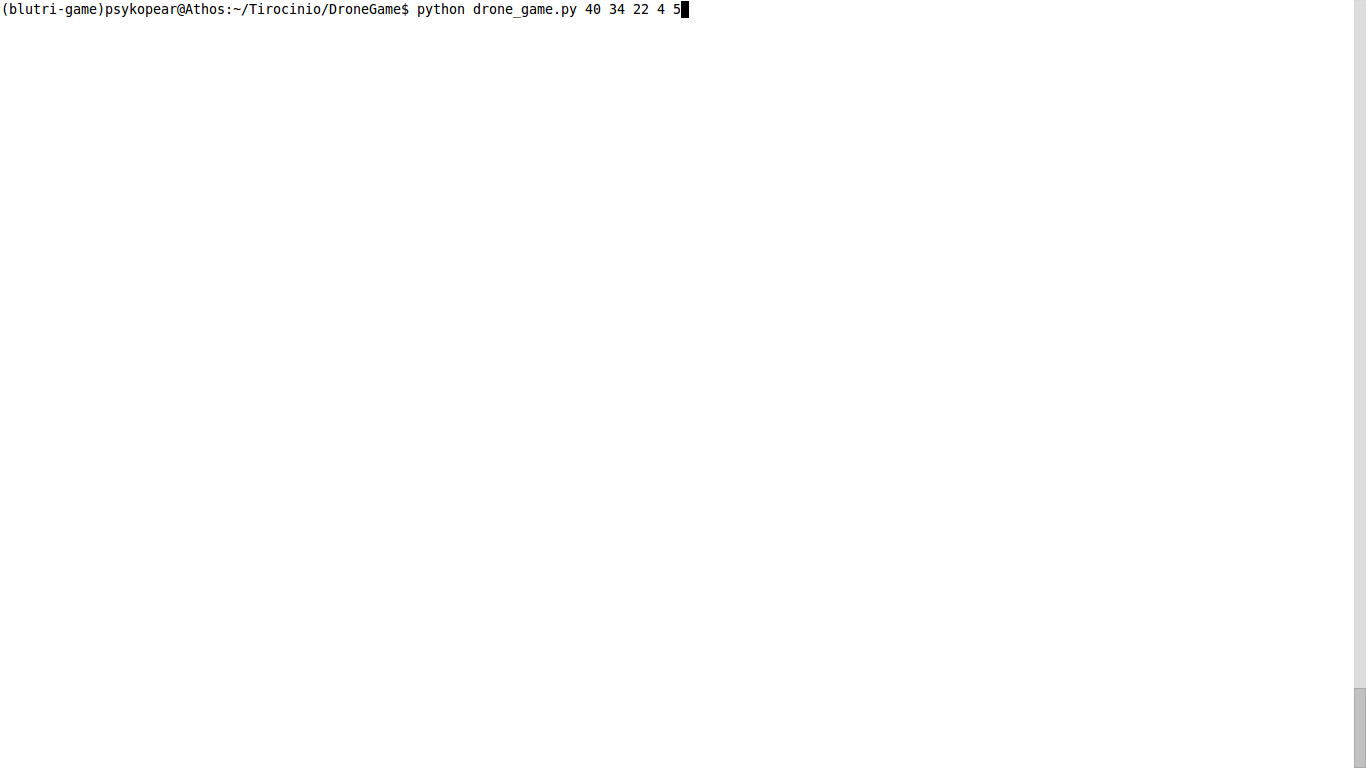
\includegraphics[width=\textwidth]{immagini/Run1.png}
\caption{Viene avviata la simulazione, su una matrice 40x40.}
\end{figure}

\begin{figure}[hb]
\center
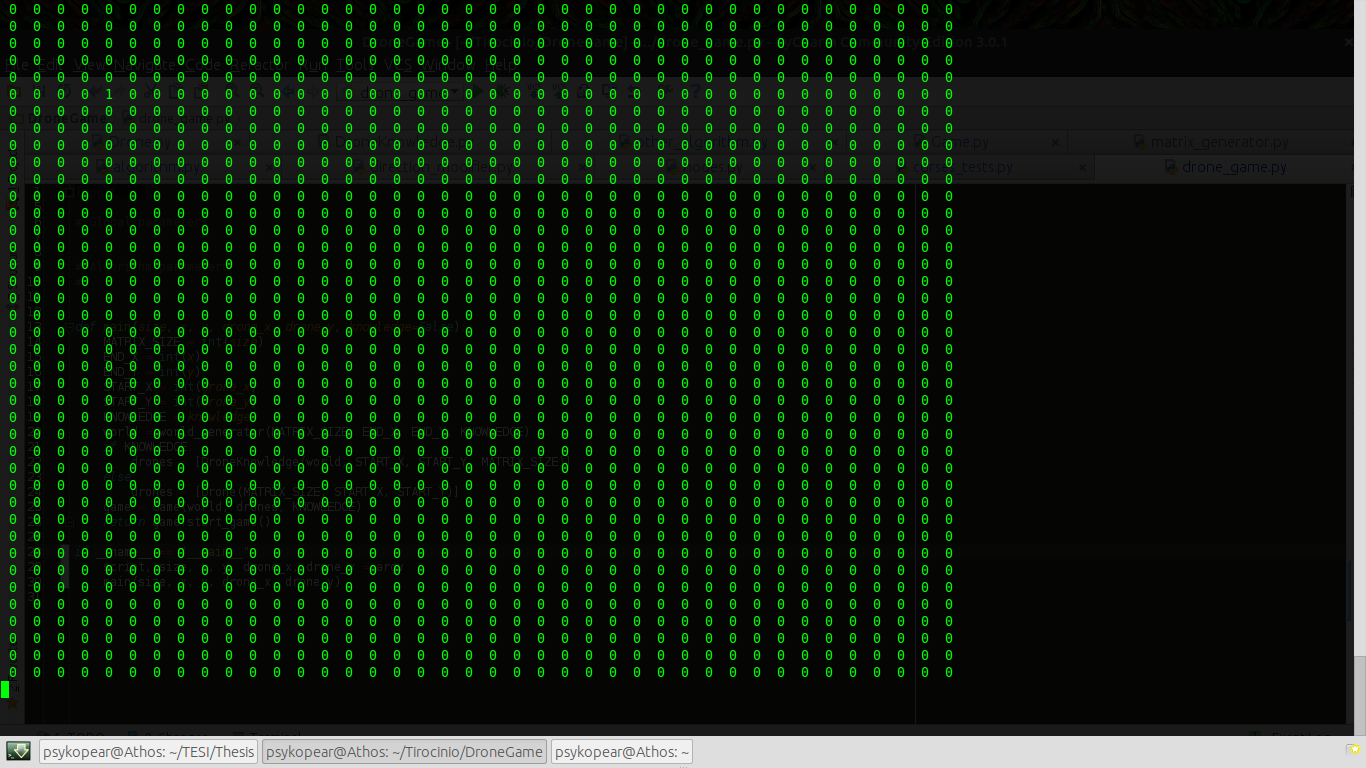
\includegraphics[width=\textwidth]{immagini/Run2.png}
\caption{Inizio: il Drone si trova dove è visualizzato il numero "1".}
\end{figure}

\begin{figure}[hb]
\center
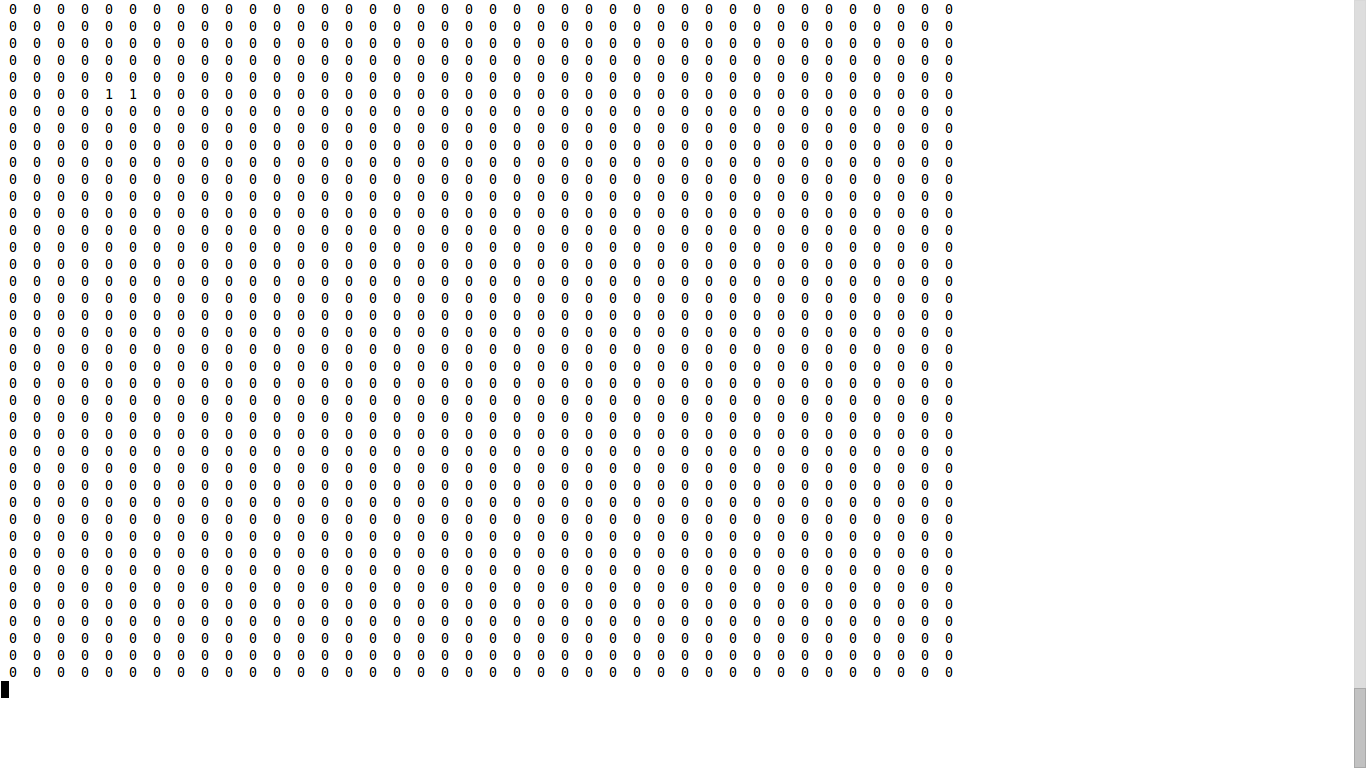
\includegraphics[width=\textwidth]{immagini/Run3.png}
\caption{Primo passo della calibrazione.}
\end{figure}

\begin{figure}[hb]
\center
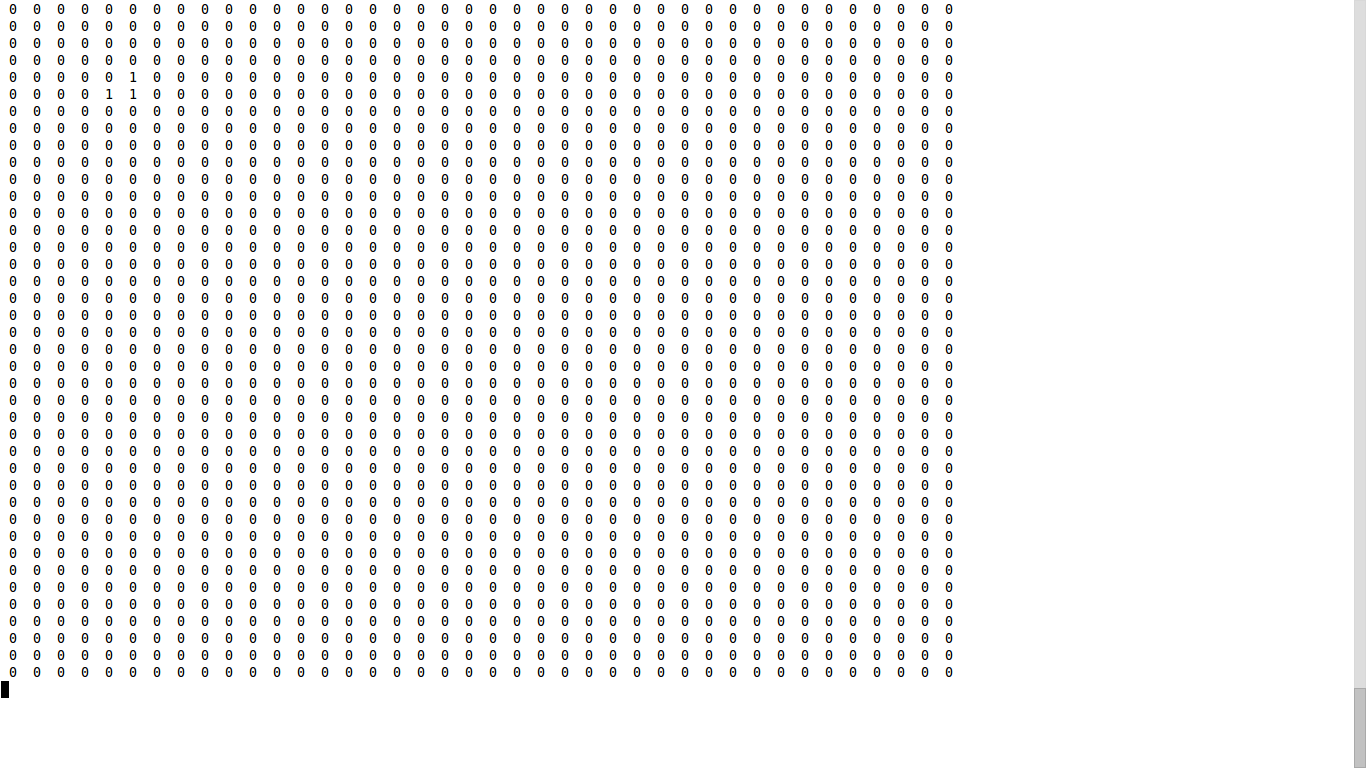
\includegraphics[width=\textwidth]{immagini/Run4.png}
\caption{Secondo passo della calibrazione.}
\end{figure}

\begin{figure}[hb]
\center
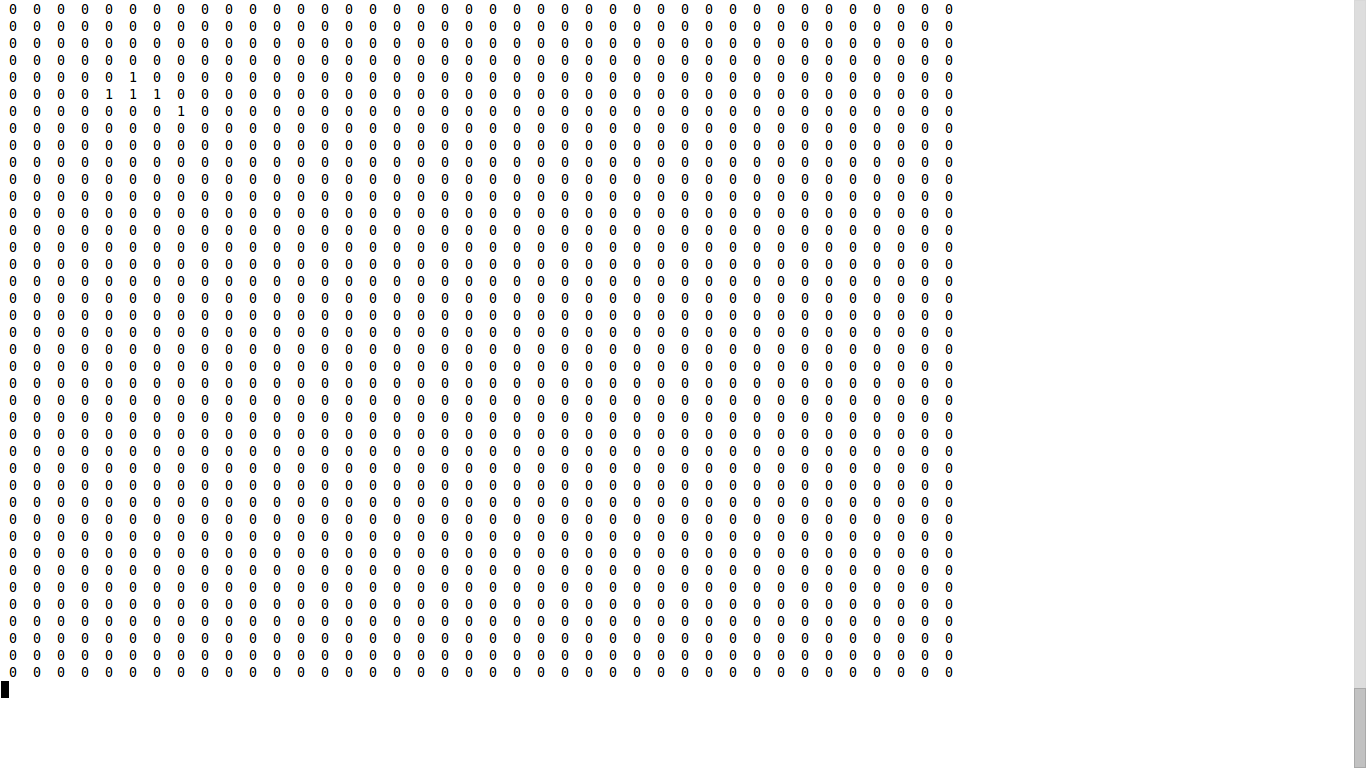
\includegraphics[width=\textwidth]{immagini/Run5.png}
\caption{Il Drone inizia a muoversi in diagonale verso l'obiettivo.}
\end{figure}

\begin{figure}[hb]
\center
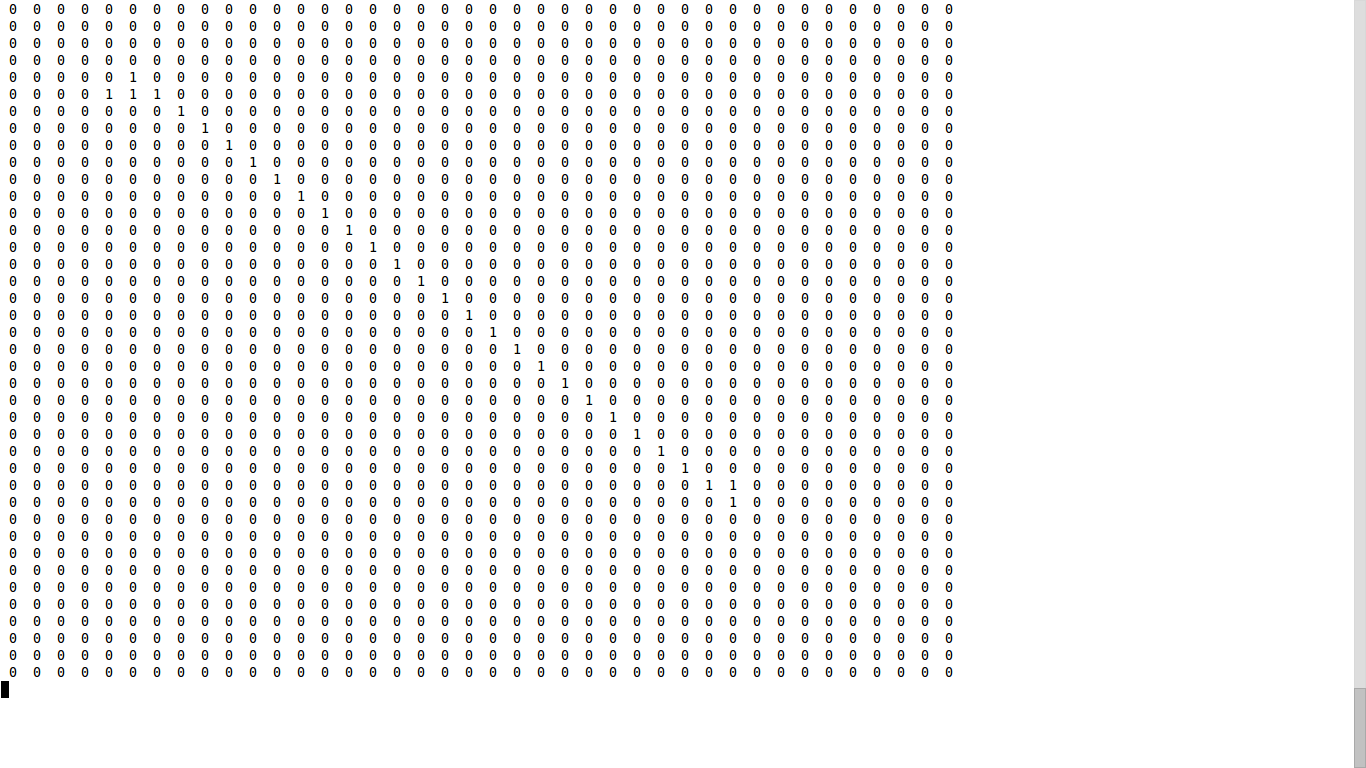
\includegraphics[width=\textwidth]{immagini/Run6.png}
\caption{Cambio direzione perchè non si sta più avvicinando.}
\end{figure}

\begin{figure}[hb]
\center
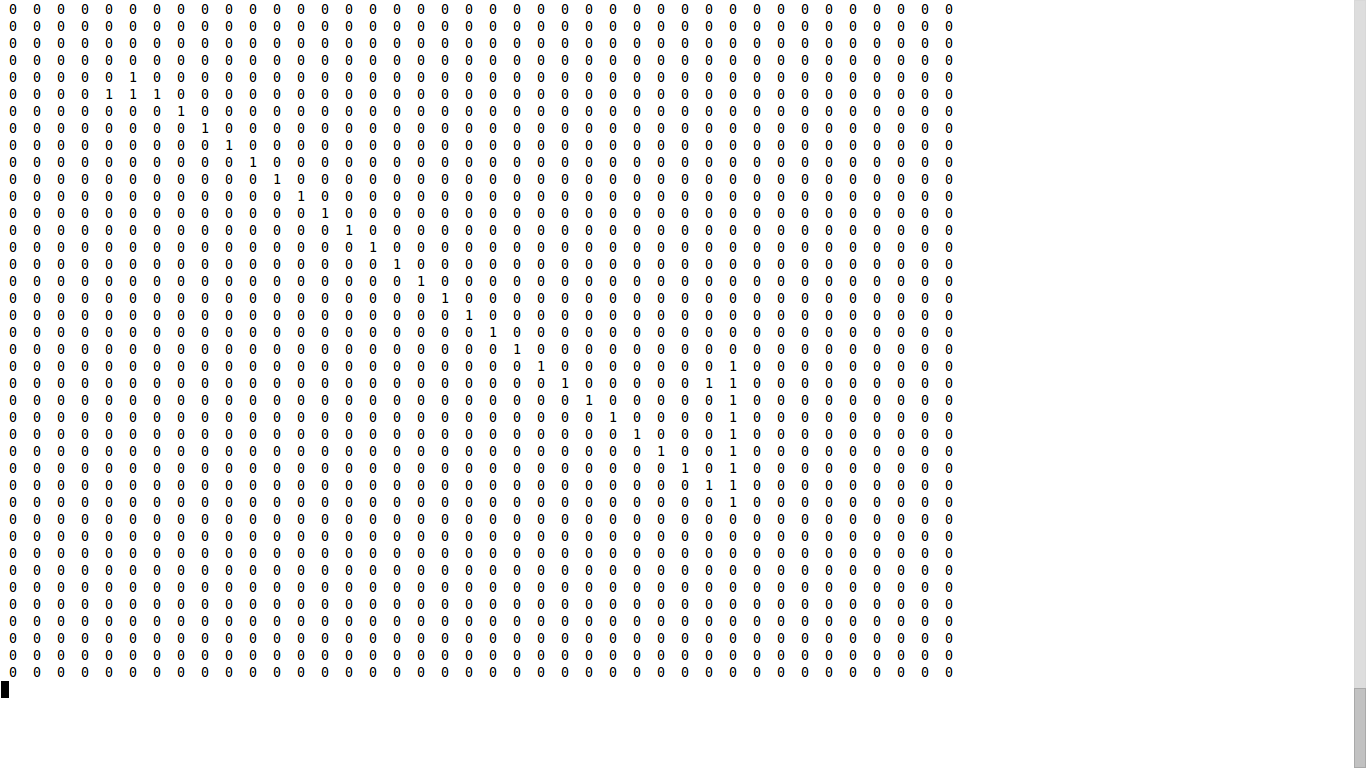
\includegraphics[width=\textwidth]{immagini/Run7.png}
\caption{Altro cambio direzione.}
\end{figure}

\begin{figure}[hb]
\center
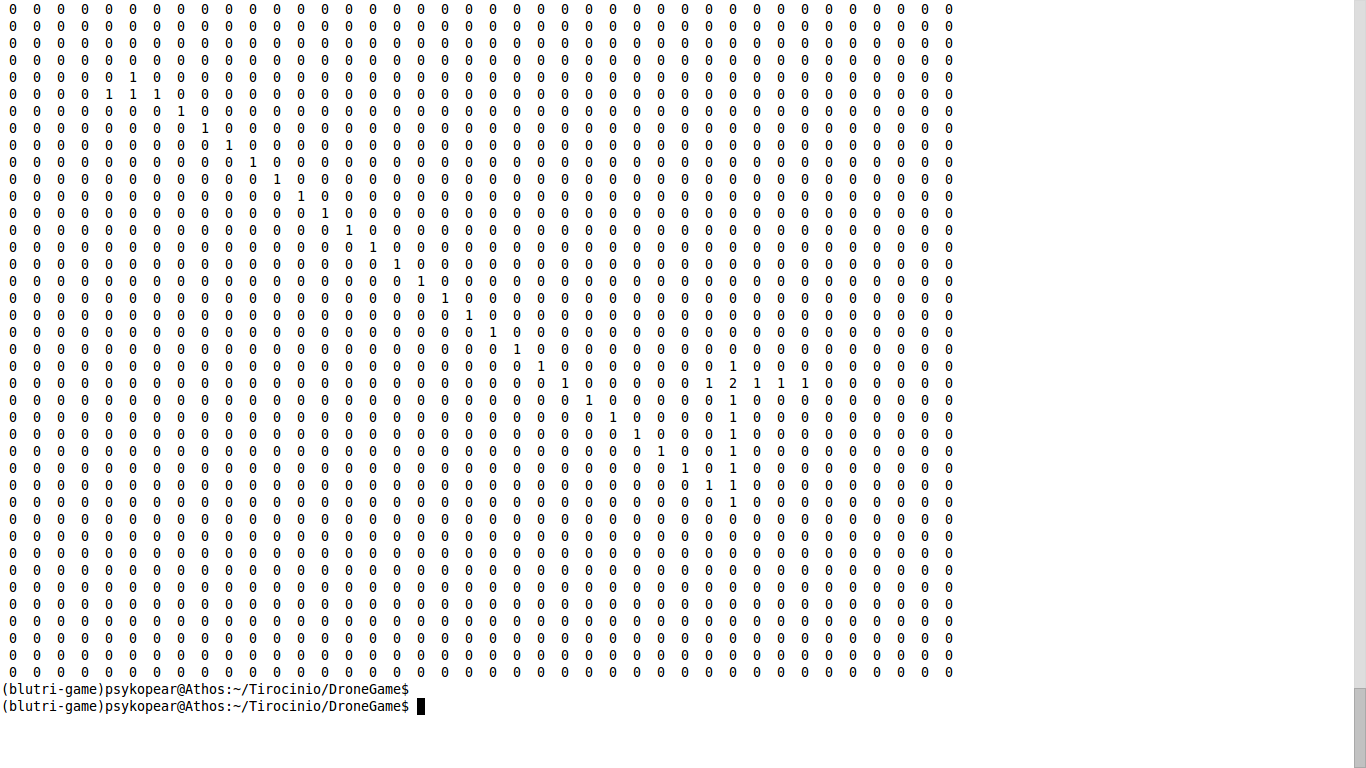
\includegraphics[width=\textwidth]{immagini/Run8.png}
\caption{Ultimo cambio di direzione ed obiettivo raggiunto.}
\end{figure}